\documentclass{article}
\usepackage{latexsym}
\usepackage[a4paper]{geometry}
\usepackage{fullpage}
\usepackage{hyperref}
\usepackage{booktabs}
\usepackage{xcolor}
\usepackage{graphicx}
\usepackage{tikz}
\usepackage[export]{adjustbox}
\usepackage{comment}
\usepackage[style=iso]{datetime2}
%\usetikzlibrary{calc}
\usetikzlibrary{arrows,positioning} 
\tikzset{
    %Define style for course boxes
    courseboxv/.style={
           rectangle,
           draw=blue!50!black, very thick,
           fill=blue!10,
           minimum height=8cm,
           minimum width=4cm,
           text width=3.9cm,
           text centered,
           font=\bfseries\sffamily},
    courseboxh/.style={
           courseboxv,
           minimum height=4cm,
           minimum width=8cm,
           text width=7.9cm},
    courseboxhh/.style={
           courseboxh,
           minimum height=4cm,
           minimum width=16cm,
           text width=15.9cm}
}
\def\frameseparation{1.5cm}
\def\scalingfactor{.9}

\newcommand{\secref}[1]{Section~\ref{sec:#1}}
\newcommand{\secreff}[2]{Sections \ref{sec:#1} and \ref{sec:#2}}
\newcommand{\eqnref}[1]{Equation~\eqref{eq:#1}}
\newcommand{\eqnreff}[2]{Equations \eqref{eq:#1} and \eqref{eq:#2}}
\newcommand{\eqnrefff}[3]{Equations \eqref{eq:#1}, \eqref{eq:#2} and \eqref{eq:#3}}
\newcommand{\figref}[1]{Figure \ref{fig:#1}} 
\newcommand{\figreff}[2]{Figures \ref{fig:#1} and \ref{fig:#2}}
\newcommand{\figrefff}[3]{Figures \ref{fig:#1}, \ref{fig:#2} and \ref{fig:#3}}
\newcommand{\tabref}[1]{Table~\ref{tab:#1}}
\newcommand{\tabreff}[2]{Tables~\ref{tab:#1} and \ref{tab:#2}}
\newcommand{\tabrefff}[3]{Tables~\ref{tab:#1}, \ref{tab:#2} and \ref{tab:#3}}

\def\year{2024--2025}
\title{EITA65 Design of Systems for Digital Transformation\\\year}
%\title{EITA65 Digitalisering -- realisering och systemdesign med användarperspektiv\\\year}
\author{\huge Databases \& Web Servers\\Raspberry Pi Project -- Part 3}
%Version \DTMnow}
\date{}

\begin{document}
\newgeometry{left=2.5cm,right=2.5cm,bottom=1.5cm}% for placing course schematic lower on first page
\clearpage\maketitle
\thispagestyle{empty}% to remove page numbering on first page

\begin{itemize}
\item This project will be done individually, but you will work \textit{together} in groups of 3 or 4.
\item You will not get detailed step-by-step instructions. Figuring out how to reach the goal is part of the project. (being a collaborative doer)
\item The results of this project part will be used in the next, so document your work.
\end{itemize}

\vspace{.1cm}
\begin{center}
\begin{tabular}{l}
\toprule[1.5pt]
\parbox{0.8\linewidth}{
\vspace{.2cm}{\Large Learning goals:}
\begin{itemize}
\item Getting hands-on experience with databases,
\begin{itemize}
\item Writing data to a database,
\item Reading data from a database,
\end{itemize}
\item Supplementing your Python toolbox.
\end{itemize}}\\
\bottomrule[1.5pt]
\end{tabular}
\end{center}

\vfill
\begin{center}
\includegraphics[width=60mm]{Database_Server.svg.png}
\end{center}
\vspace{2cm}

\begin{comment}
\begin{center}
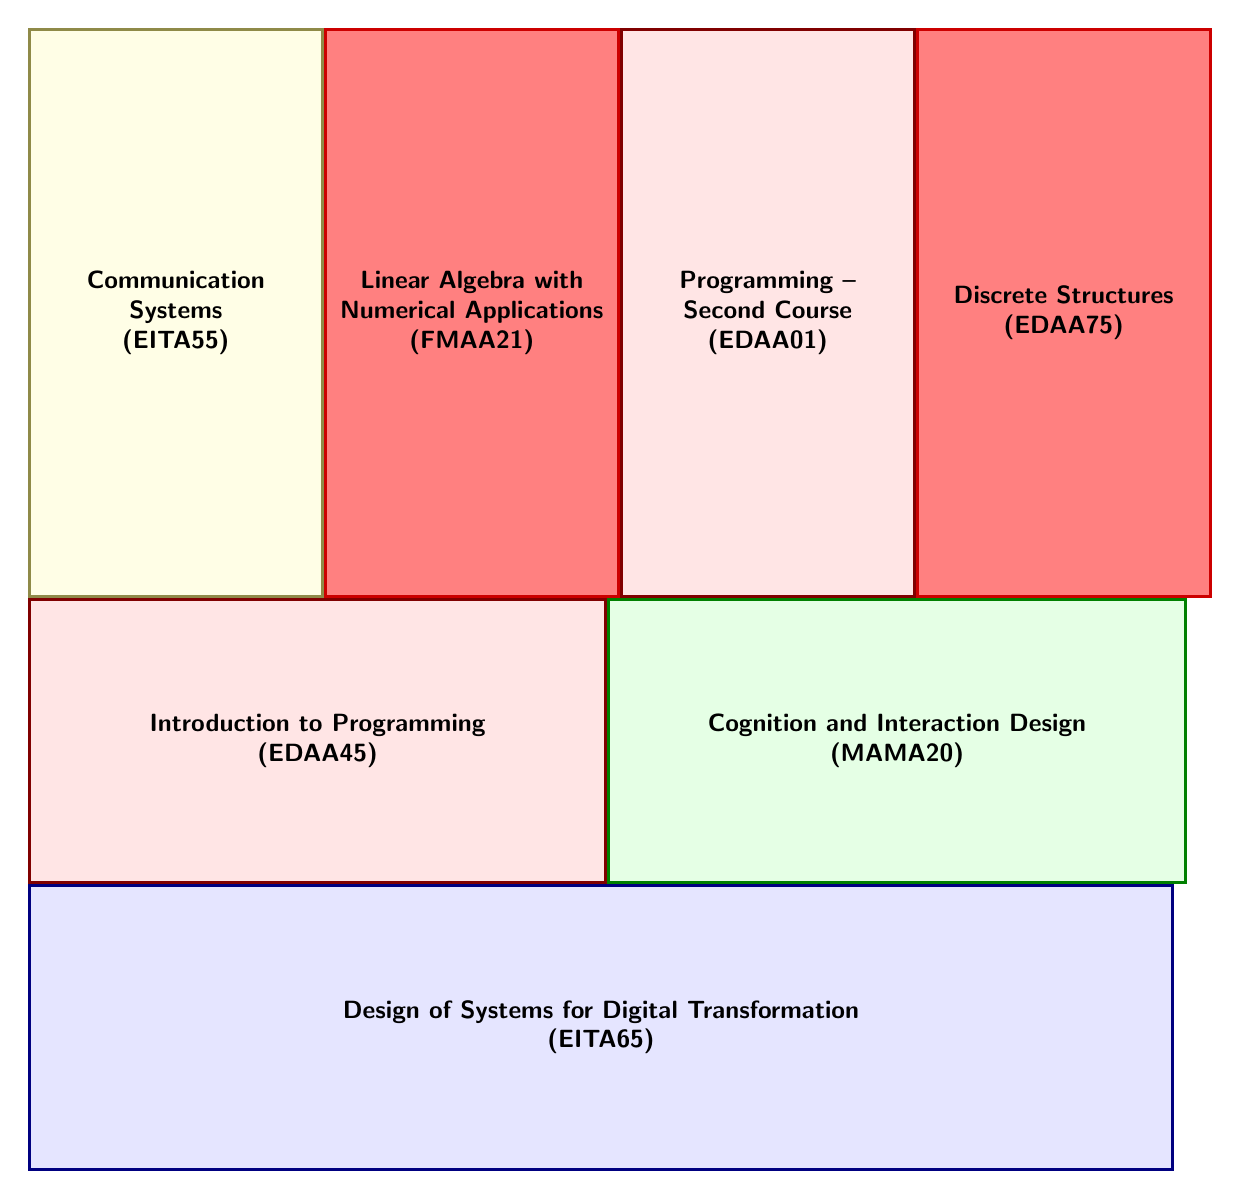
\begin{tikzpicture}[>=latex, node distance=0cm,scale=\scalingfactor,every node/.style={scale=\scalingfactor}]
\node[courseboxv, draw=yellow!50!black, fill=yellow!10] (EITA55) {Communication Systems\\(EITA55)};
\node[courseboxv, draw=red!80!black, fill=red!50, anchor=west] (FMAA21) at (EITA55.east){Linear Algebra with Numerical Applications\\(FMAA21)};
\node[courseboxv, draw=red!50!black, fill=red!10, anchor=west] (EDAA01) at (FMAA21.east){Programming -- Second Course\\(EDAA01)};
\node[courseboxv, draw=red!80!black, fill=red!50, anchor=west] (EDAA75) at (EDAA01.east){Discrete Structures\\(EDAA75)};
%\node[courseboxh, preaction={clip, postaction={fill=red!10, draw=red!50!black, line width=2mm}}, anchor=north west] (EDAA45) at (EITA55.south west){Introduction to Programming\\(EDAA45)};
\node[courseboxh, draw=red!50!black, fill=red!10, anchor=north west] (EDAA45) at (EITA55.south west){Introduction to Programming\\(EDAA45)};
%\node[courseboxh, draw=green!50!black, fill=green!10, anchor=west] (MAMA20) at (EDAA45.east){Cognition and Interaction Design\\(MAMA20)};
\node[courseboxh, draw=green!50!black, fill=green!10, right=of EDAA45] (MAMA20) {Cognition and Interaction Design\\(MAMA20)};
\node[courseboxhh, anchor=north west] (EITA65) at (EDAA45.south west){Design of Systems for Digital Transformation\\(EITA65)};
%\node[anchor=south east, inner sep=2pt, font=\bfseries\sffamily\scriptsize] at (EDA625.south east) {Helsingborg};
%\path[->,draw=black,dotted,thick] (EIT060.east) -- (EITF05.west);
%\path[->,draw=black,dotted,thick] (EIT060.south) -- (EITN50.north);
%\path[->,draw=black,dotted,thick] (EITF05.south) -- (EITN41.north);
%\draw[draw=blue!50!black, very thick] ($(EIT060.north west)+(-\frameseparation,\frameseparation)$) rectangle ($(EDA625.south east)+(\frameseparation,-\frameseparation)$);
\end{tikzpicture}
\end{center}
\end{comment}

\restoregeometry
\newpage

\section*{\huge{Database}}
\section{Introduction}
\noindent In this project part you will get acquainted with \emph{databases}. There are many different kinds of databases and we will be using one called \emph{Redis}. Redis is an acronym for \emph{Remote Dictionary Server}. Redis is comparatively easy to use with Python and has been voted most loved database in \emph{Stack Overflow Developer survey} several years in a row \cite{loved}. You will also learn how to store your sensor data in your own server!
\begin{figure}[h]
    \centering
    \includegraphics[width=20mm, trim={0 0 4.8cm 0},clip]{redis-white.png}
    \caption{Redis logo}
    \label{fig:logo}
\end{figure}
\section{How do Databases Work?}
Databases store collections of data in an organized way. Often you store information using a key, and a value. The key is unique, and the value is the information you want to store in connection to that key. For example, a civic registration number (personnummer) is often used as a key, and maybe Skatteverket would store values like tax address, age and income for all people in their database. Usually you can think of a database as a table (think excel), where the first column contains the unique key, and each row holds the values for that key.

\section{IP adresses and port numbers}

The Redis database program will run as a separate program, or \emph{service}, on your Raspberry Pi and other programs will connect to it in order to store or retrieve the data in the database. To create such a connection, the programs need a way to uniquely identify the service they want to connect to. First, we need to specify the computer on which the service is running and, second, we need to specify the particular service on that computer.

We use an \emph{IP address} to specify the computer, or \emph{host}, on which the service is running. In this exercise we will be running the Redis service on the same computer as the programs using the database and we can therefore use ''localhost'' or ''127.0.0.1'' as the IP address which means that the service runs on our local computer. You will encounter other IP addresses later in the course. If you are interested in learning more, see \cite{ipaddress}.

The \emph{port number} is a number (0-65535) identifying the service to connect to on the specified computer. Redis will by default listen to connections to port 6379, but other ports can be specified. You can find more information about port numbers at \cite{portnumber}.

\newpage

\section{Installing  and starting Redis}
To install redis on your Raspberry, use the following commands:
\begin{equation}
    \texttt{sudo apt update}
\end{equation}
\begin{equation}
    \texttt{sudo apt install redis} 
\end{equation}
By default, the Redis server will start automatically after it is installed by the command above. 
 To test if the redis server running, type the following in a terminal:
\begin{equation}
    \texttt{redis-cli ping}
\end{equation}

If it returns \texttt{PONG} in response, that means your server is already running. If not, then to start the redis server, open a new terminal, and run the command
\begin{equation}
    \texttt{redis-server}
\end{equation}
This will run the redis server on its default port 6379. If you want it to run on a different port, for example on port 7777, use
\begin{equation}
    \texttt{redis-server --port 7777}
\end{equation}
The redis server you started will run as a background process on your Raspberry and it will automatically restart when you reboot or switch on your Raspberry. The information you store in the database will remain even after you restart your Raspberry. We say the database is persistent.

To learn how to interact with Redis using a terminal, you can also follow {\color{blue}\href{https://auth0.com/blog/introduction-to-redis-install-cli-commands-and-data-types/}{this tutorial}} as an optional supplement. But for completing the project it will be enough by mastering the following notes. To test the commands in notes, type the following in a terminal:
\begin{equation}
    \texttt{redis-cli}
\end{equation}
If you did not use the standard port for your redis server, but instead for example used port 7777, type
\begin{equation}
    \texttt{redis-cli -p 7777}
\end{equation}

% \noindent {\bf Note: }\parbox[t]{14cm}{When you're checking if Redis is working, you need to use two terminals, one for the database to run in, and one to test it in.}\\
\noindent {\bf Note 1: }\parbox[t]{14cm}{To see all the keys in your database you can use the command 
}
\begin{equation}
    \texttt{KEYS *}
\end{equation}
\noindent {\bf Note 2: }\parbox[t]{14cm}{To erase all information in your database type 
}
\begin{equation}
    \texttt{FLUSHDB}
\end{equation}

\noindent {\bf Note 3: }\parbox[t]{14cm}{To create a new key-value pair, define the name and value of the key:
}
                            \begin{verbatim}
                                SET <the_key> <the_value>
                            \end{verbatim}
 
You can repeat this command with different value input for the same key name to change its value.


\noindent {\bf Note 4: }\parbox[t]{14cm}{To retrieve the value of the key:
}
                                \begin{verbatim}
                                    GET <the_key> 
                                \end{verbatim}

\noindent {\bf Note 5: }\parbox[t]{14cm}{To delete the value of the key:
}
                                \begin{verbatim}
                                    DEL <the_key> 
                                \end{verbatim}



\section{Writing and Reading Data}
In order to be able to use our database in Python, we need to install the redis \textbf{Python module}, so that we can use it to communicate with our Redis database. Use the following command to install the redis Python module:
\begin{equation}
    \texttt{sudo apt install python3-redis}
\end{equation}

\noindent
%The command \texttt{pip3} is the package installer of Python3, with which you can install, uninstall and manage all the Python modules you have on your device. We will use it a lot in our future labs, please look at \cite{pip} for more information about \texttt{pip}.

\begin{itemize}

    \item[1.] Try Redis out, using the code below:
    %{\color{blue}\href{https://amalgjose.com/2020/08/11/simple-python-program-to-connect-to-redis/}{here}}.
    \begin{verbatim}
        import redis

        # Here you connect to Redis database with its host address and port id:
        db_redis = redis.Redis( host="localhost", port=6379)

        # create a key-value pair with key as "the_key" and value as "the_value"
        db_redis.set("the_key", "the_value")

        # retrieve the value by using the key
        my_value = r_conn.get("the_key")
        print("Value from Redis: ", my_value)
    \end{verbatim}
       
    \item[2.] Store a static key-value pair (choose your own text strings) in the Redis database.
    \item[3.] Read two different kinds of sensor data value from the Sense HAT and store them in your redis database.
    \item[4.] Retrieve all the stored value from the database and print it nicely formatted.
\end{itemize}

% \section{There Can Be \textit{More} Than One}
% You can also use several\footnote{Trivia: 'There Can Be Only One' is a quote from which movie? Which famous rock group was inspired by this movie and wrote 9(!) songs for its score?} different databases in your Python program. Figure out how to make a second one available and expand what you did above as follows. A tip is to look at the \emph{Redis Quick Start}-webpage on how to install Redis more properly.
% \begin{itemize}
%     \item[1.] Store (different) static key-value pairs (choose your own text strings) in two different Redis databases.
%     \item[2.] Retrieve the stored values from the two databases and print them nicely formatted.
% \end{itemize}
% This can be useful when you want to store different kinds of data in different locations (data modeling and separation of data).

% \section{Apply to Sensor Data}
% In the drone project it can be useful to read sensor data and write them to different databases. Do the following.
% \begin{itemize}
%     \item[1.] Read two different kinds of sensor data value from the Sense HAT or the ultrasound distance detector and store them separately in your two different databases.
%     \item[2.] Retrieve the stored sensor data values from the databases and print them nicely formatted.
%     \item[3.] Modify your Python code to use a loop to repeatedly (continuously) update the sensor data values in the databases.
%     \item[4.] Modify the printing accordingly.
% \end{itemize}

\section*{\huge{Web Servers}}

\section{Introduction}
\noindent In this project part you will get acquainted with web servers and web pages. There are many different web servers. We will be using a very simple Flask server. In this part of the project you will
\begin{itemize}
\item[1.] learn how to use a Flask server,
\item[2.] create and modify web pages using HTML and CSS,
\item[3.] present sensor data on your web page.
\end{itemize}
Apart from it being easy to use, we will come back to using flask servers in the drone project.

\section{How do Web Pages and Browsers Work?}
Browsers, such as \emph{Chrome} or \emph{Safari}, are programs that find and display web pages. Web pages are \textit{hosted} on different servers, so every time you want to go to a new web page, your browser needs to communicate with the server where the new page is hosted \cite{web}. 

When you type a web address/URL (maybe \url{www.xkcd.com}) your browsers submits an HTTP request to xkcd's server, and the server starts to send over the information needed to display the web page. Your browser processes all the information which contains several different types of code (typically at least HTML, XML or JavaScript) and elements (such as Flash or ActiveX). When your browser has processed all the components, it displays the web page \cite{web}.
\begin{figure}[h]
    \centering
    \includegraphics[width=50mm]{brow.png}
    \caption{Different browser logos}
    \label{fig:logo2}
\end{figure}
\section{How do Web Servers Work?}
Web servers store web pages and all the information needed for someone to display it in their browser, and they also handle all the HTTP requests from people who want to access your web pages. You can have a server on your own computer, but normally for popular web pages, they need to use computers specifically designed to host web pages and that can handle a large number of requests for their pages and their \textit{content} \cite{serv}.

Web servers often send \textit{cookies} to your browser. Cookies are not viruses. They are simply text strings containing some information. Cookies often contain information that allows, for example, the web server to track how you have used the web page, to store settings you have used, and to keep track of which items you have put in your shopping cart \cite{cookie}. You do not need to use cookies in your web application.

\section{Flask Server}
Flask is a micro web framework that does not require any other tools or libraries. An entire lightweight web application can run in a single Python file. The name is a play on an earlier web framework called the \emph{Bottle} network \cite{bottle}.
\begin{figure}[h]
    \centering
    \includegraphics[width=50mm]{1920px-Flask_logo.svg.png}
    \caption{Flasks logo}
    \label{fig:flask}
\end{figure}

\section{Installing and using a Flask Web Server}
Flask is included in the Python3 library, and in order to try it out, follow {\color{blue} \href{https://projects.raspberrypi.org/en/projects/python-web-server-with-flask/0}{this tutorial}}. Note that Python and Flask are already installed on your Raspberry so you can ignore those steps.

In the tutorial you learned how to make a web application and how to add web pages to it. Add more pages and find more information about HTML and CSS to make your pages look better. Add at least one image to one of your pages -- use the \verb!<img>! tag to include an image object on your web page.
When you are done, your web application should consist of at least two web pages that you can navigate between (by, say, clicking on links embedded in the web pages). And your CCS styling does not need to be pretty, we are interested in you getting used to using it in practice, so any (visible) styling will do for now.\\

\noindent{\bf Note: }\parbox[t]{14cm}{When updating your CSS-file, you might need to delete your cache in your browser to be able to see the changes.}\\



\section{Lab Goal}
\textcolor{red}{In order to make everything come together, make a web page where you present your latest sensor values that you have stored in your Redis-database. If there is a new value in the database, the value should update if you refresh the page. Show your web page to the TAs.}

As a helpful hint, it is much easier (and more reasonable) if you write two scripts and run them in two terminals at the same time. The first script reads sensor data and keeps the Redis database updated with the latest reading(s), as you did in Part 5 above. You could use an infinite while loop to update the values and then sleep for, say, 10 seconds, before updating the values again. To sleep for 10 seconds import the package \texttt{time} and then do \texttt{time.sleep(10)}. The second script is your \verb!app.py!, and in the function of the web page route where you want to show your sensor data, read the data from the Redis database and pass the values as variables in the HTML code.

%\section{Theme (Optional)}
%We love music, and if you like music too, then we would love to know more about that. Please choose one of your favourite bands or artists and use that as a theme for your web page. In the impossibly unlikely event that you dislike all music ever created in the history of humankind, please let us know so we can start a fundraiser for music therapy -- and choose your own alternate theme (but extra kudos, of course, if you Rickroll \cite{rickroll} your site visitors). To add or not???





\section{Helpful Hints}

{\bf Hint 1: }\parbox[t]{14cm}{To get rid of the ugly \texttt{b''} surrounding your values you retrieve from your Redis-database, you need to use a decode method or configure your Redis connection to automatically decode any response.}\\
{\bf Hint 2: }\parbox[t]{14cm}{The value in the key-value pair does not need to be a single value. If you are up for it (it is optional), try to store data for all the Sense Hat sensors under one key.}\\
%{\bf Hint 3: }\parbox[t]{14cm}{If you want to save or open a file in Thonny that is not a \texttt{.py}-file, you have to choose \texttt{all files} in the bottom right corner of the file dialog.}\\
{\bf Hint 3: }\parbox[t]{14cm}{You do not need to worry about copyrights for images and other content that you display in you web application as long as you do not make it publicly available.}

\vspace{1cm}
\begin{center}
\huge Good luck!
\end{center}

\begin{thebibliography}{10}
\bibliographystyle{plain}
% \bibitem{iso-date-time} ISO 8601 -- Date and Time Format, \url{https://www.iso.org/iso-8601-date-and-time-format.html}, last accessed on 2021-09-21.
\bibitem{loved} Developer Survey Results 2021: Most Loved, Dreaded, and Wanted Databases, \url{https://insights.stackoverflow.com/survey/2021#section-most-loved-dreaded-and-wanted-databases}, last accessed on 2024-11-18.
%\bibitem{pip} Pip - Python package installer,  \url{https://projects.raspberrypi.org/en/projects/generic-python-installing-with-pip}.
\bibitem{ipaddress} IP Address, \url{https://en.wikipedia.org/wiki/IP_address}, last accessed on 2024-11-19.
\bibitem{portnumber} Port (computer networking), \url{https://en.wikipedia.org/wiki/Port_(computer_networking)}, last accessed on 2024-11-19.\bibitem{web} Web browser, \url{https://en.wikipedia.org/wiki/Web_browser}, last accessed on 2023-09-26.
\bibitem{cookie} HTTP cookie, \url{https://en.wikipedia.org/wiki/HTTP_cookie}, last accessed on 2021-09-29.
\bibitem{serv} Web server -- Wikipedia, The Free Encyclopedia, \url{https://en.wikipedia.org/wiki/Web_server}, last accessed on 2021-09-29.
\bibitem{bottle} Flask (web framework) -- Wikipedia, The Free Encyclopedia, \url{https://en.wikipedia.org/wiki/Flask_(web_framework)}, last accessed on 2021-09-29.
%\bibitem{rickroll} Rickroll -- Wikipedia, The Free Encyclopedia, \url{https://en.wikipedia.org/wiki/Rickrolling}, last accessed on 2021-09-30.
\end{thebibliography}

\end{document}
